\chapter{The Standard Model of particle physics}
\label{ch:theory}
\epigraph{\itshape``New ideas pass through three periods: 1) It can't be done. 2) It probably can be done, but it's not worth doing. 3) I knew it was a good idea all along!"}{--- \textup{Arthur C. Clarke}}
\mediumlinespacing
\section{Introduction}


%\hspace{10pt}\lettrine[lines=2]{\initfamily{I}}{n this day and age}, people usually tend to take for granted all, sometimes decades long, innovative efforts that were turned into every day items. It is as if this modern life style has made us suppress our natural curiosity that followed us through eons. Through its turbulent history where the fear of the unknown and the desire to understand were tightly coupled together, the human race had proven, over and over again, of being capable of choosing the side of progress. This can be seen in the current state of our scientific results which seem to be moving...

%\hspace{10pt} Looking at the timeline of the human race, by looking at the origins of first spoken proto-languages, theorised to be used to gossip or to characterise a person's qualities on top of signalling for danger. It is then baffling to see us reverting to this state of using our capacity and knowledge for the most basing needs long abandoned by our ancestors. Never ending consumption of meaningless entertainment and countless hours spent on further discussions paint a deeply concerning image of the world, where science is in desperate need of promotion.  


%* History of humans trying to understand nature\newline
%* Gossip in evolution theory\newline
%* Greek phylosophers\newline
%* Overview of modern physics\newline
%* Formation of the SM\newline

\hspace{10pt}\lettrine[lines=2]{\initfamily{T}}{he current state of particle physics} allows us to unify three out of four interactions through which our universe exists. The most complete theory that summarises this knowledge into a mathematical formalism is the Standard Model (SM). The main focus of this chapter will be to describe the main constituents of matter and how they interact with each other.

\hspace{10pt} In order to start the discussion, a short introduction on the importance of gauge theories is given before proceeding with describing details regarding each of the interactions relevant to the current state of the SM. Due to its importance to the main search presented with this thesis, special attention will be given to the Higgs mechanism and, slightly later, to the production modes of the Higgs boson itself. This chapter serves as a theoretical prelude enabling further discussion regarding the approach behind the main study, which is the focus of the next chapter.
\newpage
\section{Building blocks of the Universe}
\hspace{10pt} It is truly amazing to see that our entire physical realm can be explained through a finite set of particles. Fundamental (or elementary) particles, summarised in Tables~\ref{tab:fermions} and~\ref{tab:bosons}, can be grouped into three generations of fermions and a set of gauge bosons. Each fermion generation consists of a set of two leptons, and two quarks. The first, being comprised of the up (u) and down (d) quarks, electron and (e$^{-}$) and electron neutrino (\textnu$_\text{e}$), is responsible for all visible matter in our universe. Moving away from the stable setting towards higher energies, achieved by collider experiments, helps to complete the picture by introducing the rest. The second generation is formed by the strange (s) and charm (c) quarks accompanied by a muon and muon neutrino lepton pair, while the third is made out of top (t) and bottom (b) quarks followed with a tau lepton and tau neutrino pair.
%This completes the list of fundamental fermions, leaving one to discuss how do they all communicate with each other and how do they acquire mass.

\begin{table}[h]
    \centering
   \small
    \begin{tabular}{lccccccccc}
    \hline
           &  \multicolumn{4}{c}{Leptons} & &\multicolumn{4}{c}{Quarks} \\\cline{2-5}\cline{7-10}
       & \multicolumn{2}{c}{Particle (sym.)}  & Q & mass/GeV &  &\multicolumn{2}{c}{Particle (sym.)}   & Q & mass/GeV  \\\hline
              &  &  &  &  &  &  &  &  & \\
      First      & electron  &  (e$^{-}$) & $-1$ & 0.0005 & & down &(d)  & $-\frac{\text{1}}{\text{3}}$ & 0.003 \\
      Generation & neutrino  &  (\textnu$_{\text{e}}$) & 0 & $<\text{10}^{-\text{9}}$ & & up &(u)  & $+\frac{\text{2}}{\text{3}}$ & 0.005 \\
                    &  &  &  &  &  &  &  &  & \\
      Second      & muon  &  (\textmu$^{-}$) & $-1$ & 0.106 & & strange &(s)  & $-\frac{\text{1}}{\text{3}}$ & 0.1 \\
      Generation & neutrino  &  (\textnu$_\mu$) & 0 & $<\text{10}^{-\text{9}}$ & & charm &(c)  & $+\frac{\text{2}}{\text{3}}$ & 1.3 \\
                        &  &  &  &  &  &  &  &  & \\
      Third      & tau  &  (\texttau$^{-}$) & $-1$ & 1.78 & & bottom &(b)  & $-\frac{\text{1}}{\text{3}}$ & 4.5\\
      Generation & neutrino  &  (\textnu$_\tau$) & 0 & $<\text{10}^{-\text{9}}$ & & top &(t)  & $+\frac{\text{2}}{\text{3}}$ & 174\\
                              &  &  &  &  &  &  &  &  & \\\hline
    \end{tabular}
    \caption[Summary of fundamental fermions grouped by their respective generations (with Q denoting the electromagnetic charge expressed in units of the elementary charge).]{Summary of fundamental fermions grouped by their respective generations (with Q denoting the electromagnetic charge expressed in units of the elementary charge)~\cite{thomson_2013}.}
    \label{tab:fermions}
\end{table}

\hspace{10pt} The exchange of gauge bosons associated with each interaction (listed alongside their properties in Table~\ref{tab:bosons}) is the mechanism through which fermions communicate with each other. The most well known propagator, the photon (\textgamma) serves as the voice of the electromagnetic interaction, with the W$^{\pm}$/Z$^{\text{0}}$ bosons and gluons (g) performing the same role for the weak and strong interaction respectively.

\begin{table}[h]
    \centering
    \begin{tabular}{lcccc}
    \hline
       Interaction & \multicolumn{2}{c}{Boson} & Spin & Mass/GeV   \\\hline
        & & & & \\

       Weak  & W/Z bosons & (W$^\pm$/Z) & 1 & 80.4/91.2 \\
                       & & & & \\
      Electromagnetic & Photon & (\textgamma) & 1 & 0 \\
                & & & & \\
      Strong & Gluon & (g) & 1 & 0 \\
               & & & & \\\hline

    \end{tabular}
    \caption[Summary of gauge bosons grouped by their associated interactions.]{Summary of gauge bosons grouped by their associated interactions~\cite{thomson_2013}.}
    \label{tab:bosons}
\end{table}

\hspace{10pt} The "crown jewel" of particle physics, the Higgs boson, represents the final piece that completes the set of fundamental particles. Its mass currently stands at 125.18~$\pm$~0.16~GeV~\cite{paper:pdg} following the combined measurements performed by ATLAS and CMS collaborations.

\hspace{10pt} The importance of the Higgs field and the mechanism through which it interacts with fundamental particles will be the main point of discussion in the following sections. Further topics regarding its production modes and subsequent decays are introduced in Chapter~\ref{ch:Higgs_LHC_DM}, where the invisible final state will be explained. Currently no deviations from the SM have been observed, but, as it will be seen in the following chapters, uncertainties in these measurements leave the door open wide enough that it still motivates searches for physics beyond the SM.

\section{Introduction to gauge theories}

\hspace{10pt} The quantum mechanical Lagrangian is widely used as an essential tool in High Energy Physics (HEP) when creating a blueprint of how particles interact with each other. Further focusing on its properties, gauge theories collect the information regarding local symmetries of the given Lagrangian allowing for the introduction of symmetry groups for the Lagrangian (theory) at hand. The associated transformations of gauges lead to the formation of symmetry groups~\cite{paper:yang_mills, book:schwartz}. This as a consequence brings the fact that every group generator yields a corresponding gauge field already included in the Lagrangian due to the condition of invariance.

\hspace{10pt} From the perspective of gauge theories, the formulation of the SM is seen as a non-Abelian theory associated with: $U(1)_Y \times SU(2)_L \times  SU(3)_C$\footnote{This chapter uses the notation and conventions introduced in Ref.~\cite{thomson_2013}}. Breaking it down to core members, the $U(1)$ symmetry group is associated with the theory of Quantum Electrodynamics (QED) describing the electromagnetic interaction. The next item, the $SU(2)$ group, represents the symmetry group of the weak interaction. Finally, the Quantum Chromodynamics (QCD) theory, which focuses on the strong interaction, is connected with the $SU(3)$ symmetry group~\cite{book:group_theory, book:eliot}. The following sections introduce each of these theories in more detail. 

\hspace{10pt} Keeping with the introduction theme of this section, widely used mathematical apparatus should also be mentioned. Similarly to classical theories, the Euler-Lagrange equations can be used to obtain the equations of motion for a given theory~\cite{book:fox}. They are given as:
\begin{equation}
    \frac{d}{dt}\left ( \frac{\partial \mathcal{L}}{\partial \dot{q_i} } \right ) - \frac{\partial \mathcal{L}}{\partial q_i} =0,
\end{equation}
where $q_i$ and $\dot{q_i}$ represent generalised coordinates and corresponding velocities for the given theory. The symbol $\mathcal{L}$, denoting the Lagrangian density, is going to be referred to in further text simply as the Lagrangian.

\hspace{10pt} Another helping hand comes in the form of Noether's theorem~\cite{paper:noether}. The main statement originating from it, regarding the Lagrangian at hand, is the existence of a conserved current connected to the respective symmetry. 

\section{Quantum electrodynamics}
\hspace{10pt} Starting from the quantum mechanical generalisation of Einstein's energy-momentum relation, an expression denoting the Klein-Gordon equation can be written. Expressed in its Lorentz-invariant formulation, it takes the form of:
\begin{equation}
    (\partial_{\mu}\partial^{\mu}+m^2)\psi = 0,
\end{equation}
where the $\partial_\mu$ denotes the partial derivative (with the summation of repeating indices being imposed as a convention)~\cite{thomson_2013,book:schwartz}. The plain wave solutions of the aforementioned equation prove problematic when it comes to the interpretation of its negative energy solutions, which also arise from the original relation. The problematic nature is manifested in the fact that this scenario yields a probability density that has the possibility of being negative in value.

\hspace{10pt} An alternative approach was taken by Dirac, leading to the formulation of the Dirac equation. Its covariant form, as well its Lagrangian, can be written as:

\begin{equation}
    i\gamma^{\mu}\partial_{\mu}\psi-m\psi = 0,
\end{equation}
\begin{equation}
\mathcal{L} = i\overline{\psi}\gamma^{\mu}\partial_{\mu}\psi  - m\overline{\psi}\psi,
\end{equation}

The generalisation of the aforementioned Lagrangian to the QED leads to the following definition:
\begin{equation}
    \mathcal{L}_{QED} = i\overline{\psi}\gamma^{\mu}\partial_{\mu}\psi  - m\overline{\psi}\psi - \frac{1}{4} F^{\mu\nu}F_{\mu\nu} + e\overline{\psi}\gamma^{\mu}\psi A_{\mu},
\end{equation}

where $A^{\mu}$ represents the electromagnetic four-potential and $F^{\mu\nu} = \partial^{\mu}A^{\nu}-\partial^{\nu}A^{\mu}$ denotes the electromagnetic field strength tensor. The addition of two new terms (representing the kinetic term for $A_{\mu}$ and the interaction term respectively) allows for the fulfillment of Maxwell's equation, which can be obtained through the use of the Euler-Lagrange equations with respect to $A^{\mu}$~\cite{book:bjorken_qed, book:bjorken_qft}.

\hspace{10pt} This Lagrangian is invariant under the $U(1)$ local symmetry, or in other words, it remains unchanged with respect to the transformations: $\psi^{'}(x) = e^{-i\epsilon\lambda(x)}\psi(x)$ and $A^{'}_{\mu} = A_{\mu} + \partial_{\mu}\lambda$ (where the later corresponds to the choice of the Lorentz gauge). The redefinition of the partial derivative: $D_{\mu} = \partial_{\mu} - ieA^{\mu}$ leads to the following expression for the QED Lagrangian:

\begin{equation}
        \mathcal{L}_{QED} = i\overline{\psi}\gamma^{\mu}D_{\mu}\psi  - m\overline{\psi}\psi - \frac{1}{4} F^{\mu\nu}F_{\mu\nu},
\end{equation}

The previously written Lagrangian captures the basis of QED, whose formulation was awarded a Nobel prize~\cite{nobel_qed}.


\section{Quantum chromodynamics}
\hspace{10pt} Similarly to the development of QED and its connection to the $U(1)$ symmetry group, the origin of QCD is strongly connected to the initial introduction of isospin and the formation of an isospin doublet comprised of a proton and neutron. Further development led to a better understanding of the non-elementary structure of protons and neutrons, paving way for the currently used quark model. QCD is associated with the $SU(3)$ symmetry group, whose generators give rise to eight gluon fields~\cite{thomson_2013,book:schwartz, gell_mann}. %Additional extensions to principles applied to QED are found, such as the existence of three colour charges (connected to the nature of the symmetry group itself). 

\hspace{10pt} The local local phase transformations of the $SU(3)$ group can be written as: $\psi^{'} = e^{ig_{s}\lambda_a(x) T_a}\psi$, where the generators of the SU(3) group are defined as $T_a = \frac{1}{2}t_a$ (with the $t_a$ being the Gell-Mann matrices). The QCD Lagrangian can now be formulated in the following way:

\begin{equation}
    \mathcal{L}_{QCD} = i\overline{\psi}\gamma^{\mu}D_{\mu}\psi - m\overline{\psi}\psi - \frac{1}{4}G_{a}^{\mu\nu}G^{a}_{\mu\nu},
\end{equation}

where the covariant derivative takes the form of: $D_{\mu} = \partial_{\mu} + igT_aG^{a}_{\mu}$, with $G_{\mu}^a$ representing the gluon fields and  $G_a^{\mu\nu}$ denoting field strength tensors. In the previous scenario the index $a$ indicates the existence of eight fields being connected to the $SU(3)$ generators. Finally, these generators do not possess the commutation property of QED, making QCD a non-Abelian theory~\cite{book:guenther}.
\section{Electroweak interaction}
\label{sec:ew_unification}
\hspace{10pt} In contrast to the previously discussed theories, a model describing the weak interaction is required to take an approach which accommodates the observed violation of parity. The aforementioned requirement led to the formulation of the V-A (vector and axial vector coupling) structure~\cite{book:eliot}. 

\hspace{10pt} The initial theory of weak interactions was associated with the $SU(2)_L$ symmetry group and the weak isospin ($I_W$), where the $L$ denotes the behavior of charged-current in which it can only be implicated with left handed particles~\cite{thomson_2013, book:schwartz}. The transformations of the weak isospin doublet $\psi^{'} = e^{ig_W\lambda_a(x)T^a}\psi$\footnote{With $T_a$ being the generators of the $SU(2)$ group.} (and the accompanying redefinition of the partial derivative as $D_\mu = \partial_{\mu}+ig_WT_aW_\mu^a$) leads to the appearance of three gauge fields $W_\mu^a$, from which the $W^{\pm}$ fields can be formed as:
\begin{equation}
    W^{\pm} = \frac{1}{\sqrt{2}}(W_\mu^1\mp iW_\mu^2).
\end{equation}
\hspace{10pt} The journey towards electroweak unification begins with the properties of QED. A massive undertaking by Glashow, Salam and Weinberg (GSW)~\cite{glashow,salam,weinberg} was formulated into the GSW model whose starting point begins with the introduction of the weak hypercharge ($Y$), through the use of the following relation:
\begin{equation}
    Q = I_W^3+\frac{1}{2}Y,
\end{equation}
where $Q$ represents the electromagnetic charge and $I_W^{3}$ denotes the third component of $I_W$. The, now $U(1)_Y$, symmetry group of QED brings the transformation $\psi^{'} = e^{ig^{'}\frac{Y}{2}\lambda(x)}\psi$ and a field $B_{\mu}(x)$ associated with it. The interpretation arising from the GSW model is that the Z boson and photon associated fields are linear combinations of the, previously introduced, $W^{3}_{\mu}$ and $B_{\mu}$:

\begin{equation}
    Z_{\mu} = -B_{\mu}\sin\theta_W + W^3_{\mu}\cos\theta_W,
\end{equation}  
\begin{equation}
    A_{\mu} = B_{\mu}\cos\theta_W + W^3_{\mu}\sin\theta_W.
\end{equation}

The summary of the GSW model is the conclusion that the unified electroweak interaction is represented by the $SU(2)_L\times U(1)_Y$ symmetry group. The corresponding Lagrangian can be written as:

\begin{equation}
    \mathcal{L}_{EW} = i\overline{\psi}\gamma^{\mu}D_{\mu}\psi - \frac{1}{4}B^{\mu\nu}B_{\mu\nu} - \frac{1}{4}W^{\mu\nu}_aW^a_{\mu\nu},
    \label{eq:ew_unification}
\end{equation}

where $D_\mu = \partial_\mu+ ig^{'}B_{\mu}\frac{1}{2} + ig_WW_{\mu}^aT_a$ and $B_{\mu\nu}$ and $W_{\mu\nu}^a$ represent field tensors for $B_{\mu}$ and $W_{\mu}^a$ respectively.

\section{Brout-Englert-Higgs mechanism}
\hspace{10pt} Following the discovery of the Higgs boson at the experiments within the Large Hadron Collider (LHC), the revolutionary nature of the Brout-Englert-Higgs (BEH) mechanism~\cite{brout, higgs} was recognised and awarded the Physics Nobel prize in 2013~\cite{nobel_beh}. Its base idea follows the spontaneous symmetry breaking approach which can be introduced by taking a look at a simple scenario of a Lagrangian of a scalar field defined as:

\begin{equation}
    \mathcal{L} = \frac{1}{2}(\partial_{\mu}\phi)(\partial^{\mu}\phi) - \frac{1}{2}\mu^2\phi^2 - \frac{1}{4}\lambda\phi^4.
\end{equation}

Omitting the kinetic term of the aforementioned Lagrangian and focusing only on the potential, a conclusion arises that there can be two distinct scenarios depending on the values of the $\mu^2$ parameter\footnote{The $\lambda$ parameter is already constrained by having to be positive in order for the potential to have a global minimum.}~\cite{thomson_2013,book:schwartz}. Figure~\ref{fig:higgs_potential} shows the shapes of the given potential (denoted as $V(\phi)$) for both the $\mu^2<0$ (marked in blue) and $\mu^2>0$ (marked in red) scenarios.

\begin{figure}[!htbp]
  \centering
    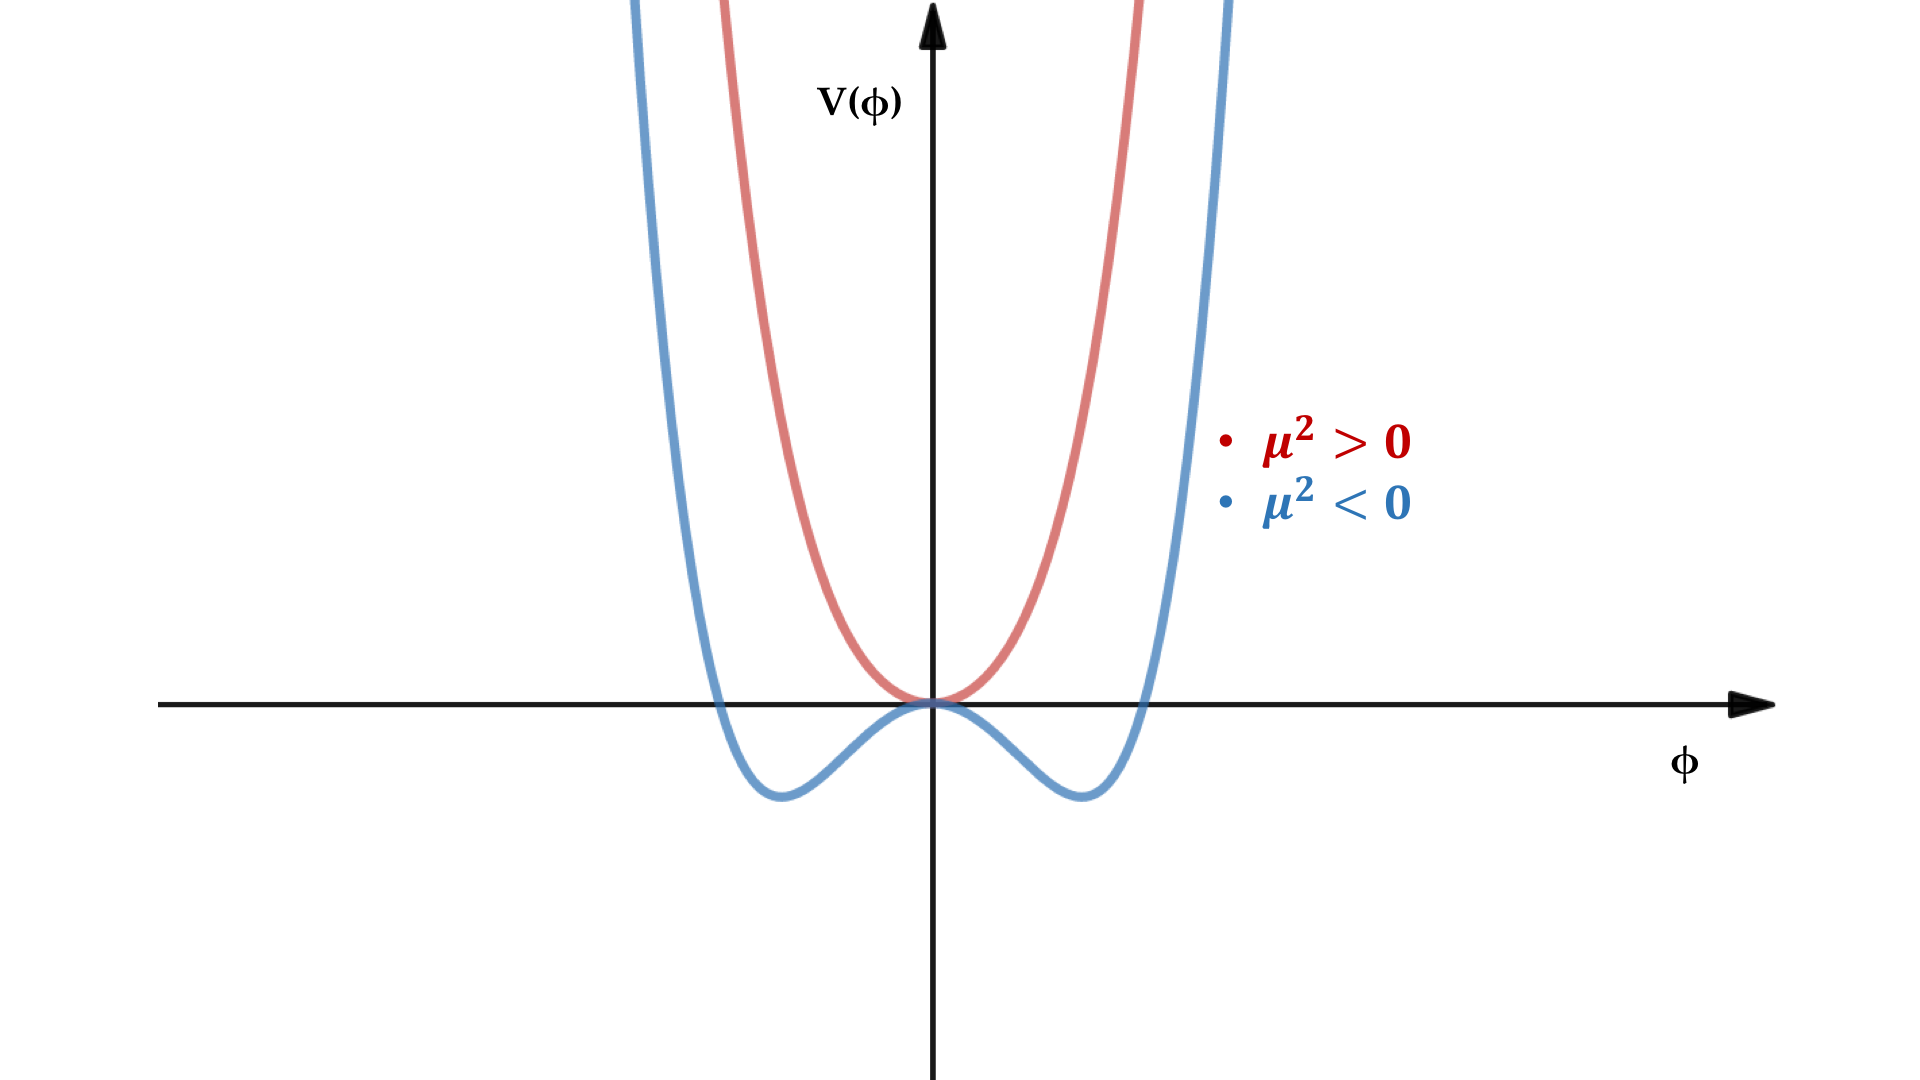
\includegraphics[width=\textwidth]{Theory/Higgs.png}
  \caption{Graphical representation of the potential $V(\phi) = \frac{1}{2}\mu^2\phi^2 + \frac{1}{4}\lambda\phi^4$ for both the $\mu^2<0$ (blue) and $\mu^2>0$ (red) scenarios (made using Ref.~\cite{desmos}). }
  \label{fig:higgs_potential}
\end{figure}

Taking the look at the first derivative in order to find the local extrema:

\begin{equation}
    \frac{\partial V}{\partial \phi} = \mu^2\phi + \lambda \phi^3 = 0,
\end{equation}

leads to the scenarios of $\phi_a = 0$ (for the $\frac{\partial^2 V}{\partial \phi^2} = \mu^2>0$) and $\phi_b = \pm|\sqrt{-\frac{\mu^2}{\lambda}}|$ (for the $\frac{\partial^2 V}{\partial \phi^2} = -2\mu^2>0$ or the $\mu^2<0$ case). The symmetry breaking of the Lagrangian happens when a choice between the two values of $\phi_b$ are made (in further text renamed as $v = |\phi_b|$). Expressing $\phi$ in terms of its vacuum expectation state, one can introduce $H(x)$ and rewrite the Lagrangian as:
\begin{equation}
    \phi(x) = v+H(x),
\end{equation}
\begin{equation}
    \mathcal{L} = \frac{1}{2}(\partial_{\mu}H)(\partial^{\mu}H) - \frac{1}{2}\mu^2(v+H)^2 - \frac{1}{4}\lambda(v+H)^4.
\end{equation}

Grouping of terms quadratic in $H(x)$ leads to its mass term within the Lagrangian, or in other words: $m_{H} = \sqrt{-2\mu^2}$.

\hspace{10pt} A natural extension leads to the inclusion of a complex version of the aforementioned potential with $\phi = \frac{1}{2} (\phi_1+i\phi_2)$ and $V(\phi) = \mu^2\phi^*\phi+\lambda(\phi^*\phi)^2$. Repeating the search for global minimum leads to the possible choice of a vacuum state of $\phi_{vac} = (v, 0)$ and the re-composition of $\phi$ as: $\phi = \frac{1}{2}(v+H(x)+i\chi(x))$. As a second step in the process, a good way to evolve the simplified Lagrangian is to take a look at the U(1) gauge symmetry. This can be done by using the kinetic term with the appropriate re-definitions of the partial derivative (as done in Section~\ref{sec:ew_unification} for $B_{\mu}$) as well as using the choice of the unitary gauge in order to remove the $\chi$ dependency\footnote{This can be achieved by choosing $\lambda(x) = -\frac{1}{g^{'}v}\chi(x)$}. This new Lagrangian, when rewritten in terms of $H(x)$, yields a massive scalar field, the Higgs field, associated with $m_{H}$ alongside a massive gauge boson (associated with $B_{\mu}$) and the appropriate interaction and self interaction terms.

\hspace{10pt} Lastly, this approach is to be applied to the $SU(2)_L\times U(1)_Y$ symmetry group, as previously defined in Section~\ref{sec:ew_unification} closely associated with the unified electroweak interaction. This requires a re-definition of $\phi$ through a weak isospin doublet and the usage of the Lagrangian defined with Equation~\ref{eq:ew_unification}. Following the procedure of searching for a global minimum, applying the unitary gauge and expanding the Lagrangian in terms of $H(x)$ gives a similar, yet slightly more complex picture. Grouping the mass terms for the appropriate fields ultimately yields:
\begin{equation}
m_W=\frac{1}{2}g_Wv,~ m_Z = \frac{v}{2}\sqrt{g^{'2}+g_W^2}~\text{and}~m_A = 0\footnote{Where the latter two are obtained through the diagonalization of the mass matrix as explained in great detail in Ref.~\cite{thomson_2013}.}.
\end{equation}

\hspace{10pt} Before concluding this part of the story, there is one more topic that needs to be addressed and that is the mechanism through which fermions acquire their mass. In order to add an item corresponding to the mass term of fermions within the electroweak Lagrangian, it has to be invariant under $SU(2)_L\times U(1)_Y$ transformations. For the $I_W^3 = -\frac{1}{2}$ fermions this term can be written as:

\begin{equation}
\mathcal{L} = -g_f(\overline{L}\phi R+ \overline{R}\phi^{\dagger}L),
\end{equation}

where $g_f$ denotes the Yukawa coupling and $L$ ($R$) represents the SU(2) doublet (singlet). Through the process of spontaneous symmetry breaking, upon rewriting the Lagrangian in terms of $H(x)$, it can be seen that the fermion masses can be associated with the Yukawa coupling as:
\begin{equation}
    m_f = \frac{vg_f}{\sqrt{2}}
\end{equation}

\hspace{10pt} After the introduction to the SM presented here, the following chapter will connect the advancements made in collider physics with the potential for beyond the SM physics through the idea behind the invisible decays of the Higgs boson. 
%\chapter{Higgs Boson and collider experiments}
\chapter{When Higgs boson met dark matter}
\epigraph{\itshape``Nothing in life is to be feared, it is only to be understood. Now is the time to understand more, so that we may fear less."}{--- \textup{Marie Curie}}
\label{ch:Higgs_LHC_DM}
\section{Introduction}


\hspace{10pt}\lettrine[lines=2]{\initfamily{B}}{eing the main focus} for studies covered by this thesis, special attention needs to be given to the Vector Boson Fusion production mode of the Higgs boson, while also discussing other topologies interesting for the invisible final state. Upon completing this discussion, a slight turn in focus is going to be taken in order to introduce the current understanding of the term dark matter (DM). It is presented alongside the investigation of a possible connection between DM searches and measurements of properties of the Higgs boson performed at hadron collider experiments. This will culminate with the illustration of the analysis idea for probing of the SM through the invisible final state of the Higgs boson decay. Finally, in order to complete the whole picture a brief overview of previously obtained results is presented.


\section{Production modes of the Higgs boson}
\label{sec:prod_higgs}
\hspace{10pt} The main interest of the two general purpose experiments centered around the interaction points of the LHC~\cite{LHC_TDR} (consequently for this thesis as well) is the production and subsequent decays of the Higgs boson. Figure~\ref{fig:higgs_prod_diag} shows diagrams for its various production mechanisms relevant for hadron colliders, in this case the proton-proton collisions (more details about the experimental setup are given in Chapter~\ref{ch:cms_experiment}).

\begin{figure}[htbp]
    \begin{center}
        \subfigure[$ggH$]{
        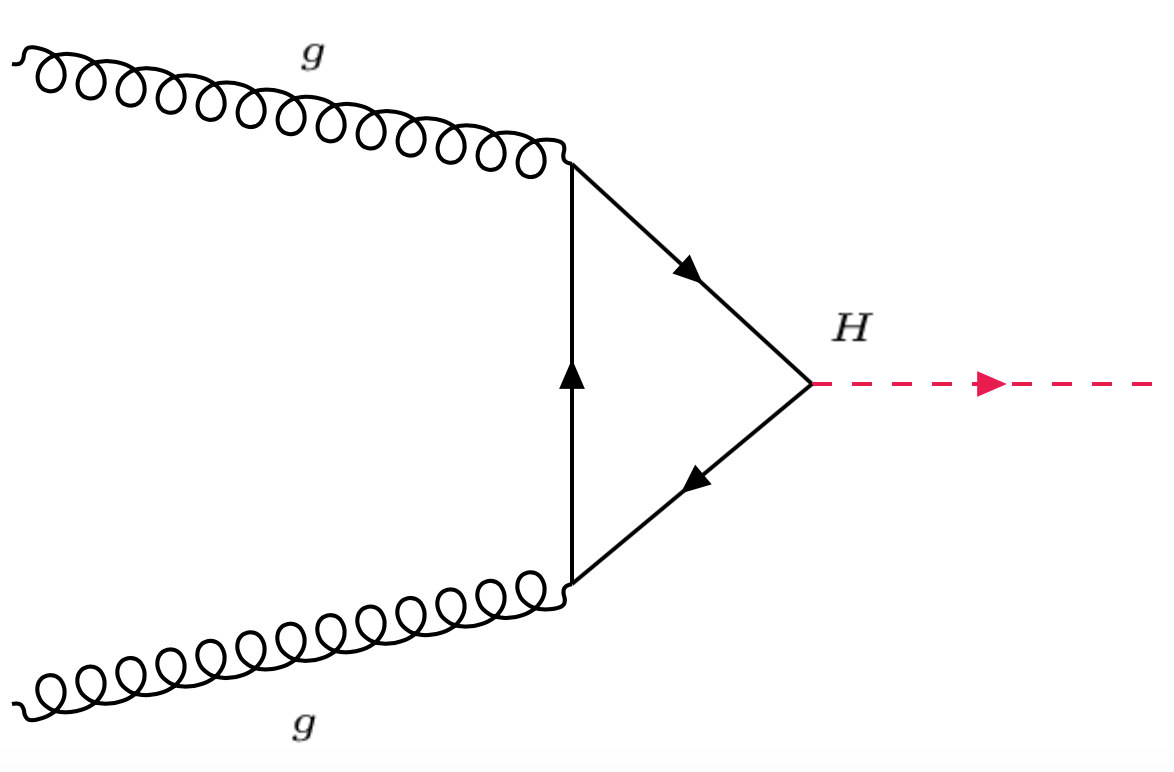
\includegraphics[width=0.45\textwidth]{Theory/ggH.png}}
        \subfigure[$qqH$]{
        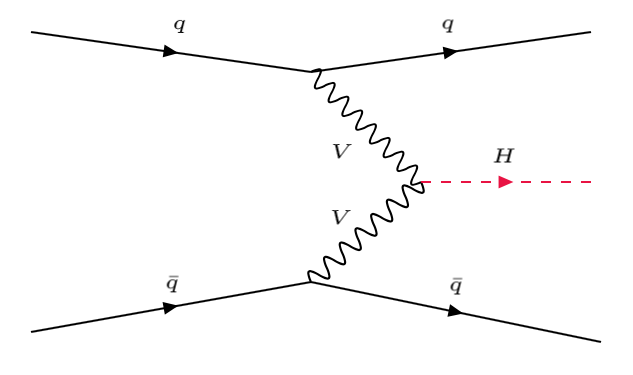
\includegraphics[width=0.45\textwidth]{Theory/vbf.png}}\\
        \subfigure[$VH$]{
        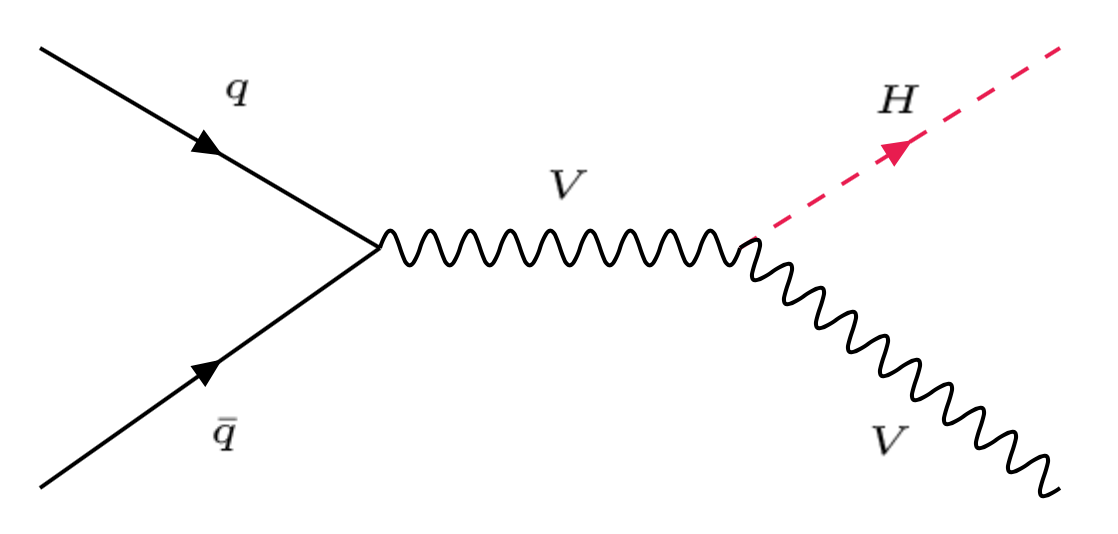
\includegraphics[width=0.45\textwidth]{Theory/VH.png}}
        \subfigure[$ttH$]{
        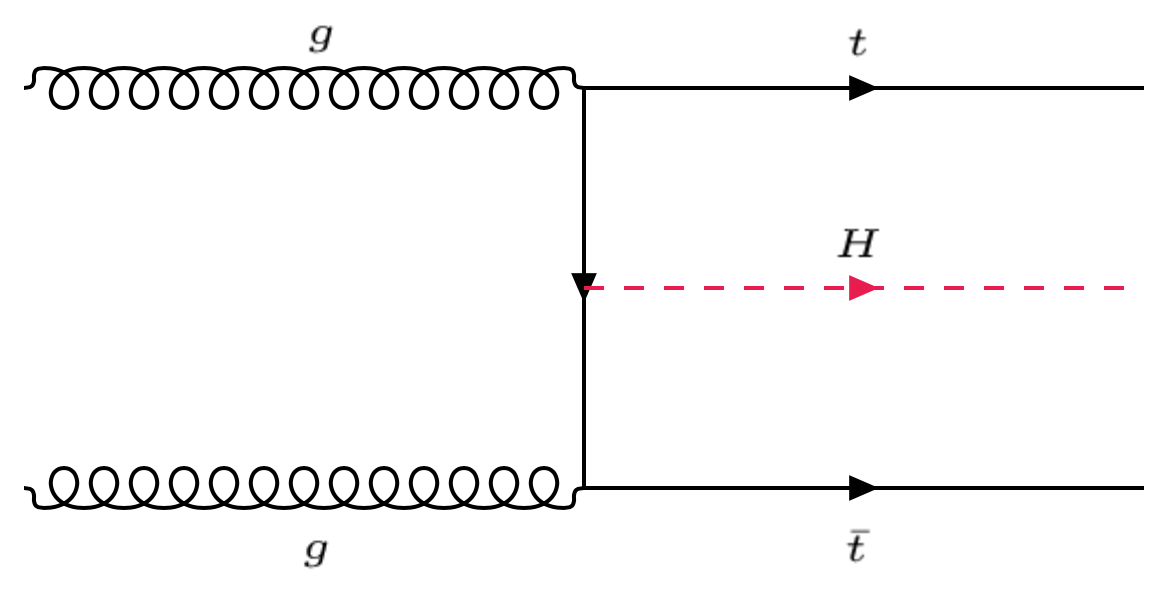
\includegraphics[width=0.45\textwidth]{Theory/ttH.png}}    
        \caption{Diagrams for the main production mechanisms of the Higgs boson: a) gluon gluon fusion, b) Vector Boson Fusion, c) Higgs-strahlung and d) associated production with top quarks (diagrams were made using Ref.~\cite{fey_diag}).}
      \label{fig:higgs_prod_diag}
    \end{center}
  \end{figure}

\hspace{10pt} The production mode with the largest cross section is the gluon-gluon fusion (ggH)~\cite{paper:ggH1,paper:ggH2}, where jets\footnote{A collimated stream of hadrons.} can arise due to initial state radiation (ISR)\footnote{Leading to a reduction of the production cross section (subsequently its importance), but still being relevant to these studies.}. The production of a Higgs boson proceeds through, as the name suggests, a gluon fusion forming a virtual quark loop which ultimately yields the aforementioned boson. The production mode with the second largest cross section, but the highest importance for this thesis, is the Vector Boson Fusion (qqH or simply VBF) mechanism~\cite{paper:ggH1,paper:ggH2,paper:vbf1,paper:vbf2}. The collision enables an exchange of virtual vector bosons which fuse together to produce a Higgs boson. This leaves a Higgs+2 jets scenario, where the jets are located close to the beam line. There is no color exchange between these jets. From the perspective of the plane perpendicular to the beam line, jets have a small separation due to the production of the Higgs boson. This distribution is mostly flat in shape as a direct reflection of the nature of Higgs boson's coupling to vector bosons~\cite{paper:higgs_dphijj}. Lastly, its main properties involve a large dijet invariant mass as a direct consequence of the large jet separation. Having defined these two production modes, it is good starting point for the introduction of the main focus of this thesis.  The search for the invisible (from the experimental point of view) decays of the Higgs boson explores a possibility of physics beyond the SM being present in one of the decay modes of the Higgs boson. The main idea behind the study relies of the, previously introduced, distinct features of the VBF prodction mode, coupled with a strategy to quantify the invisible contribution from the perspective of the experiment at hand. As this strategy relies on the Higgs+2 jets scenarios, there will be a significant contribution originating from ggH processes, which also can produce a 2 jet final state, and populate the low dijet invariant mass ranges. For the analysis described in this thesis, the combination of both the VBF and ggH+2 jets scenarios is referred to as signal.

\hspace{10pt} Continuing with other production modes, the Higgs strahlung or the associated VH production~\cite{paper:vh} happens when the colliding particles produce a virtual vector boson which can emit a Higgs boson. Lastly, a Higgs boson can be produced in association with top quarks~\cite{paper:tth1,paper:tth2}. Figure~\ref{fig:hig_production_xs} shows the production cross sections for these scenarios ranging over various proposed masses of the Higgs boson, serving as an illustrative example of the order of importance for the SM Higgs boson.

\begin{figure}[htbp]
    \begin{center}
        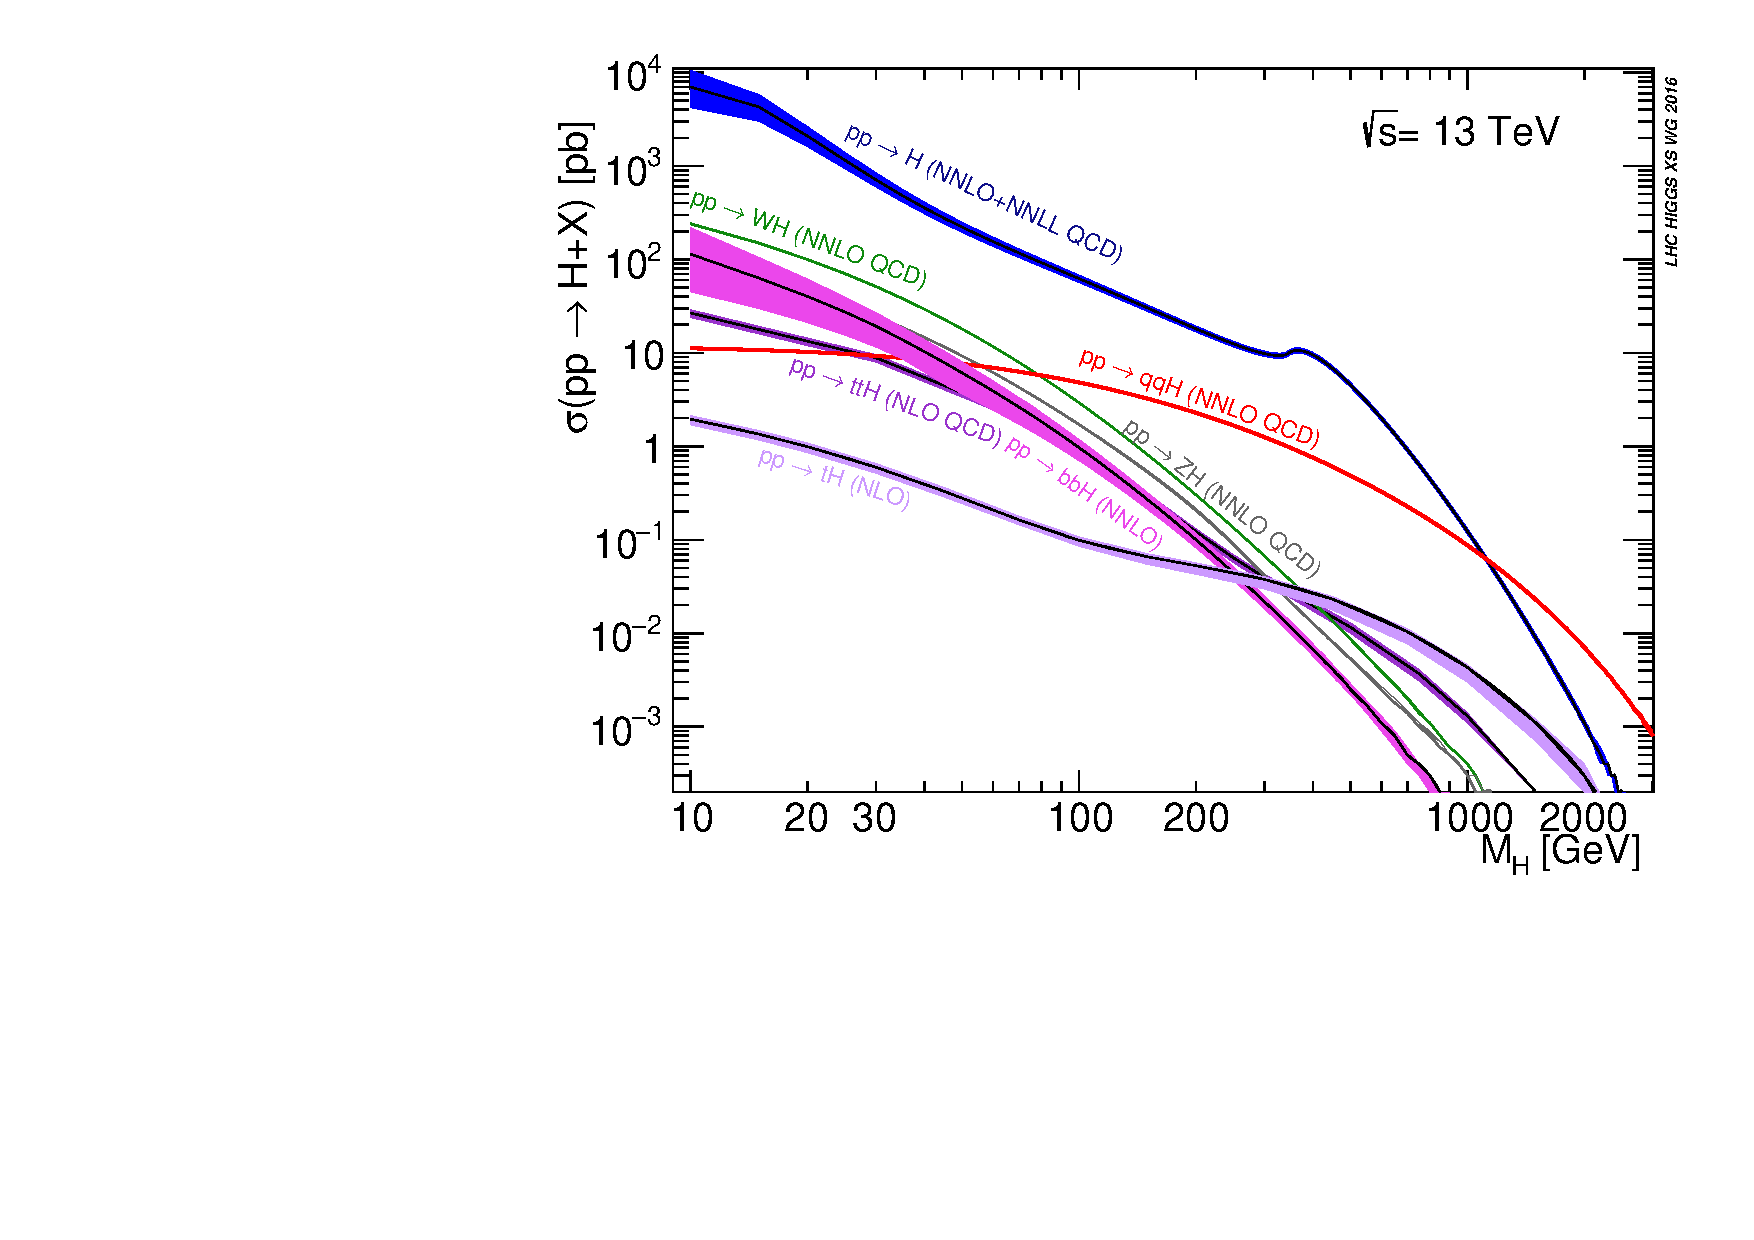
\includegraphics[width=0.8\textwidth]{Theory/higgs_prod_13TeV.pdf}  
        \caption{Cross sections for various production mechanisms of the Higgs boson originating from proton-proton collisions at the energies of $\sqrt{s}=$~13~TeV~\cite{twiki:lhcxswg}.}
      \label{fig:hig_production_xs}
    \end{center}
  \end{figure}

\hspace{10pt} The measurements of properties of the Higgs boson, which followed its discovery by the Large Hadron Collider experiments~\cite{paper:higgs_discovery1,paper:higgs_discovery2}, show a good agreement with the SM~\cite{paper:higgs_prop1,paper:higgs_prop2,paper:higgs_prop3}, but the uncertainties on these measurement are not yet small enough to fully exclude the possibility of physics beyond the SM. The current generation of collider experiments is not able to reach the O(MeV) range of precision needed to test the $\Gamma_{SM}^H$ (the total decay width of the Higgs boson predicted by the SM), leaving an indirect way of testing for beyond the SM physics\footnote{Within the area of physics concerned with Higgs boson decays.} with only one other option - to make use of results arising from measurements of the visible final states in order to set an upper limit on the beyond the SM branching ratio. Using the measurements of the visible final states as well as assuming the $\Gamma_{SM}$ leads to the result where this approach yields an 95\% Confidence Level (CL) upper limit on the branching ratio of the Higgs boson to invisible final state\footnote{More details about this approach, alongside with a detailed introduction to the $\kappa$ framework is given in Ref.~\cite{report_lhcxswg_3}} of Br(H$\rightarrow$inv)$~\sim$~0.34~\cite{paper:higgs_prop1}. From the SM point of view the only viable decay leaving the invisible signature is H$\rightarrow$ZZ$\rightarrow$4$\nu$, which has a negligible probability of happening (with Br(H$\rightarrow 4\nu )\sim$~0.1\%). This all calls for a more detailed approach through a dedicated VBF H$\rightarrow$inv search which can further improve the given limit for the branching ratio for the invisible final state.

% Figure~[R] further expands on this discussion showing the results of combined measurements from CMS and ATLAS collaborations expressed in terms of the coupling factors $\kappa_X$ (the corresponding model being introduced in Ref.~[R]), where the $k =$ 1 denotes agreement with the SM\footnote{The $\kappa_X$ facttors are intrdoced as additional multipliers to the coupling constants of the Higgs to the respective particles found in the final state. When the value of $\kappa_X=$~1 it states that no modification of the SM predicted coupling constant is needed.}


\section{Invisible final state}
\hspace{10pt} The interest surrounding final states involving particles invisible to hadron collider detectors is due to the potential beyond the SM physics hiding within their cloak. From the perspective of studies involving the Higgs boson properties, the SM predicts that the fully invisible decay is highly suppressed with Br(H~$\rightarrow4\nu$)~$\sim$~0.1\%~\cite{report_lhcxswg_3}, making it a good option for testing for beyond the SM physics. As mentioned in the previous section, the limiting factors arising from the indirect searches create motivation for this, more direct, approach~\cite{paper:hinv_run1,paper:HIG_17_023,Patrick,Riccardo}. Connection to DM searches can be found in Higgs portal theories~\cite{paper:hig_portal_models1,paper:hig_portal_models2,paper:hig_portal_models3,paper:hig_portal_models4}, where the Higgs boson can take the role of a mediator between the particles from two sectors (SM and DM), but more about those in the following section. In order to be able to approach this invisible final state with current detectors, the Higgs boson is required to recoil against a visible system.

\hspace{10pt} The production mode bringing the most sensitivity to this final state is the VBF where, as introduced in Section~\ref{sec:prod_higgs}, the Higgs boson is associated with two jets. From the SM side, there are a few processes which can mimic the exact final state of interest and those are mostly originating from V+jets processes (where V denotes W or a Z boson). Their contribution can be categorised into reducible or irreducible. The completely irreducible scenario is found when the Z boson decays to two neutrinos (the Z~$\rightarrow\nu\nu$ decay) and for the W~$\rightarrow l\nu$ case (where the charged lepton has been missed in the detection process). Example diagrams showing both the strong and electroweak modes of production (in further text referred to as QCD and EWK modes) of a Z boson decaying to neutrinos are shown in Figure~\ref{fig:znunu_diagram}. 

\begin{figure}[htbp]
    \begin{center}
        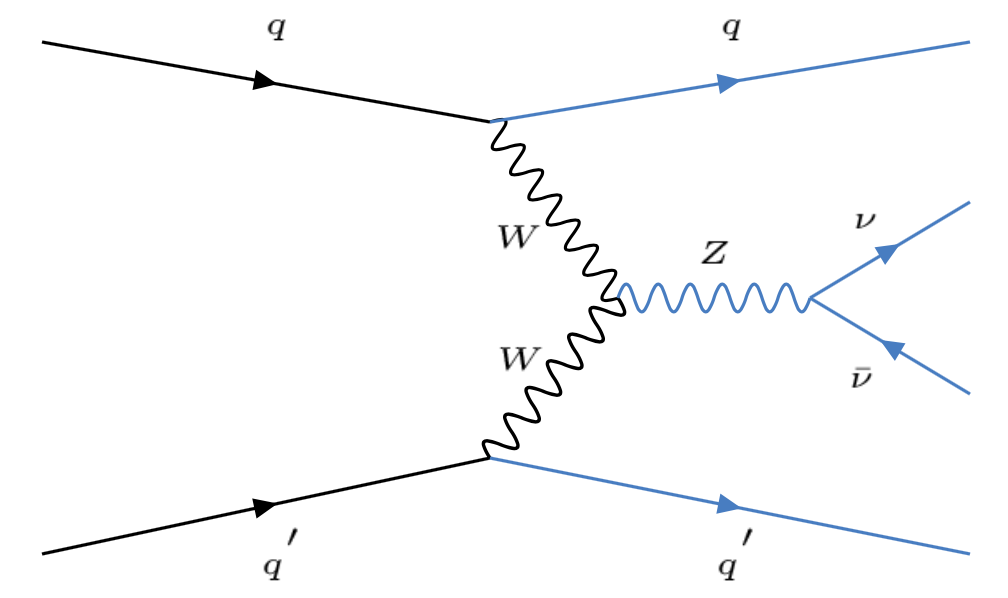
\includegraphics[width=0.47\textwidth]{Theory/ewk_znunu.png}
        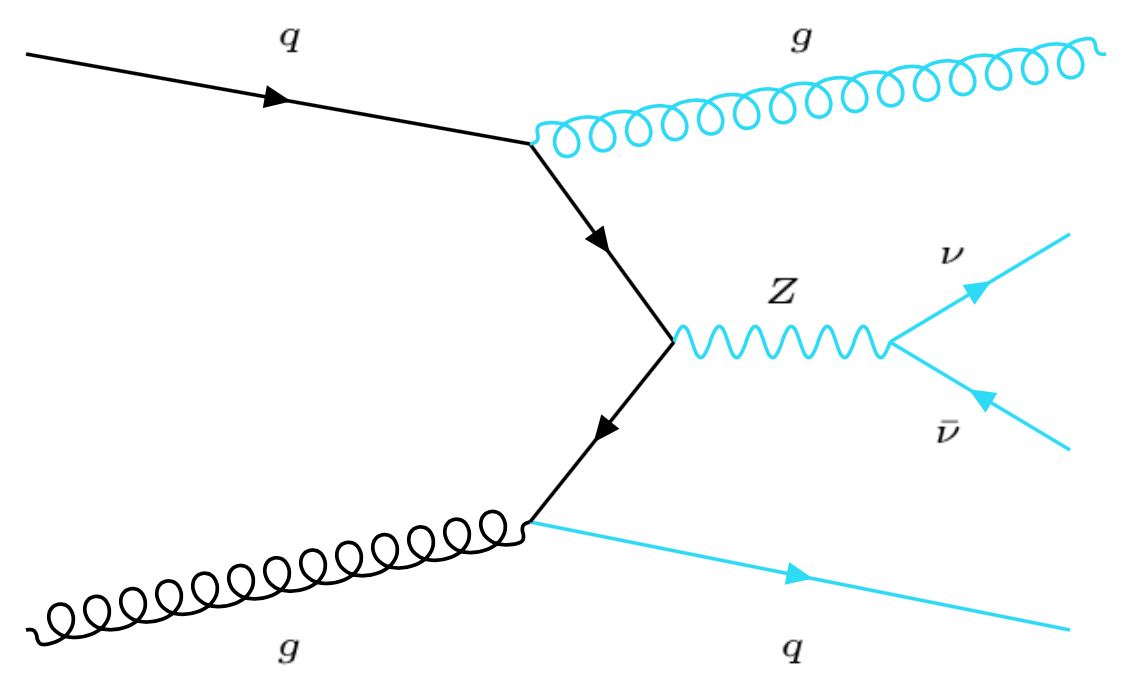
\includegraphics[width=0.47\textwidth]{Theory/qcd_znunu.png}
        \caption{Feynman diagrams for two main $Z\rightarrow \nu\nu$ irreducible background SM processes shown for both the EWK (left) and QCD (right) production modes at leading order (colors assigned to final states follow the choice used to mark the corresponding processes in further chapters). The diagrams were made using Ref.~\cite{fey_diag}.}
      \label{fig:znunu_diagram}
    \end{center}
  \end{figure}


\hspace{10pt} An additional background contribution can arise from strong multijet processes, which due to their large production rate can produce a sizeable contribution which mimics the desired final state. The estimation of the contribution originating from these main irreducible background processes is the focus of Chapter~\ref{ch:control_regions} where data driven methods are deployed. Additional minor contributions, which can arise from diboson (VV) and top quark ($t\overline{t}$ and single top) processes, are estimated through the use of simulated samples of respective processes.

\section{The dark connection}
\label{sec:dm}
\hspace{10pt} With all the great knowledge regarding particle physics currently written down as the SM, it still does not account for all of the matter in the universe. Many cosmological observations suggest that there exists another form of matter which does not posses an affinity towards the electromagnetic interaction - dark matter~\cite{intro_dm}. Following the current cosmological model, it is categorised that $\sim$~5\% of the universe's mass-energy is visible matter, 27~\% dark matter and 68\% dark energy~\cite{paper:dm_composition}.

\hspace{10pt} The most commonly used observation illustrating this is the appearance of a discrepancy in the distributions of rotation velocities of spiral galaxies when comparing the predicted result (which assumes they are comprised only from visible matter) to what is observed in reality. This is illustrated in Figure~\ref{fig:DM}, where the observed velocity distribution $V_C(Radius)$ (with its corresponding fit), represented with points (solid line), is compared with the visible matter only approach (dashed lines denoting disk and gas contribution) alongside a DM halo contribution (dashed line with the point) accounting for the missing piece~\cite{paper:dm_vc}. This can be expanded with a list of other studies such as the ones focusing on galaxy clusters~\cite{paper:dm_gal_clust} and gravitational lensing~\cite{paper:dm_grav_lens}.

\begin{figure}[htbp]
    \begin{center}
        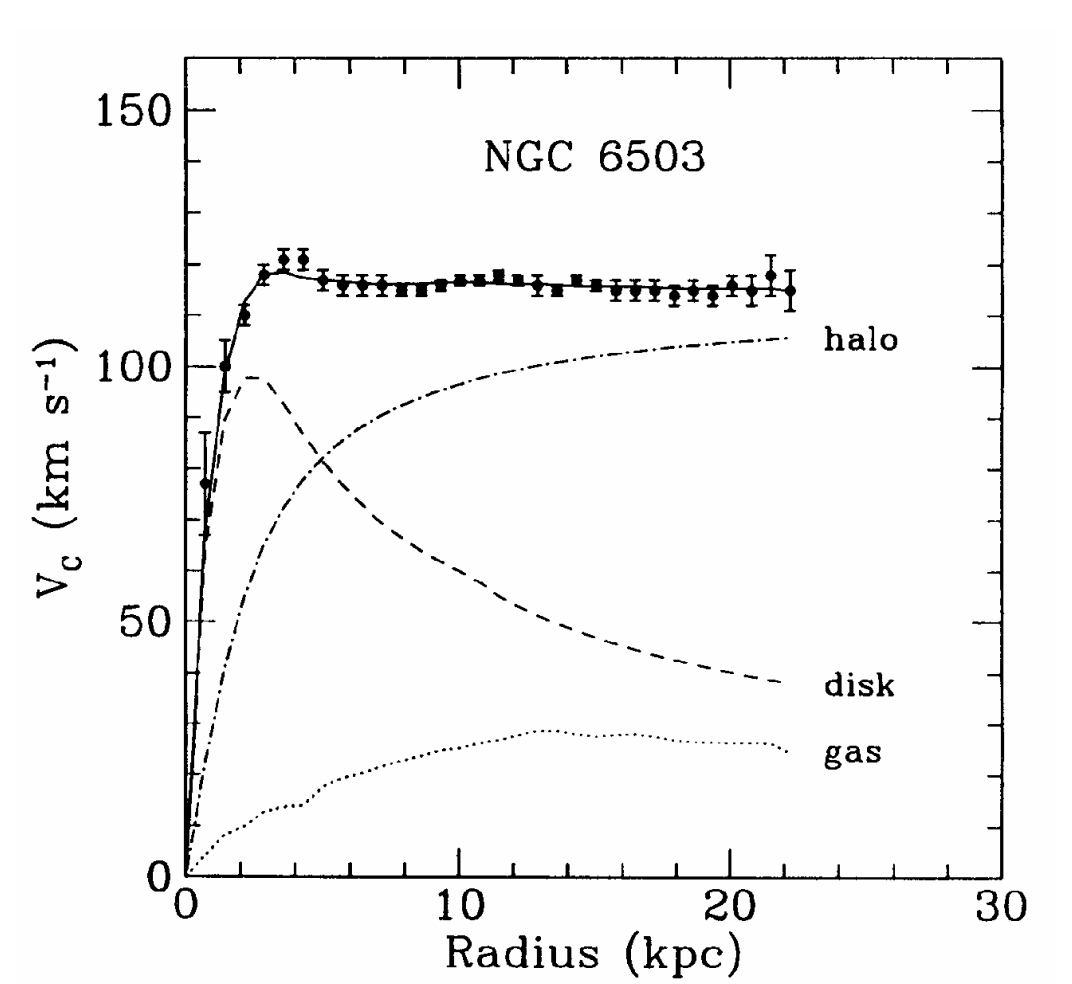
\includegraphics[width=0.7\textwidth]{Theory/DM_velocity.png}
        \caption{The distribution of the rotation velocity for the NGC 6503 is presented as an example of cosmological observation of DM~\cite{paper:dm_vc}.}
      \label{fig:DM} 
    \end{center}
  \end{figure}



\hspace{10pt} Staying in the area relevant to the theme of this thesis, the potential candidates for particles comprising the invisible final state discussed above can be associated with the DM sector. This would require a modification of the SM Lagrangian to include terms which enable the coupling of the Higgs boson to the particles from the DM sector. These can include one of the following scenarios~\cite{paper:hinv_run1, paper:hig_portal_models1,yellow_report}:
\begin{equation}
    \mathcal{L}_{S} = -\frac{1}{4}g_{HSS}H^\dagger H S^2,~\mathcal{L}_{V} = \frac{1}{4}g_{HVV}H^\dagger HV_\mu^\dagger V^\mu~\text{and}~\mathcal{L}_{f} = \frac{1}{4}g_{H\chi\chi}H^\dagger H\overline{\chi}\chi
\end{equation}
where $\mathcal{L}_{S}$ shows the (quartic) interaction term connecting the SM Higgs doublet with the DM sector, this time being represented with a scalar type ($S$). The equivalent definitions stand for the latter two terms with the scalar DM field being replaced with a vector ($V$) and a fermion ($f$) type, respectively.

%\hspace{10pt} The following sections introduce the statistical approach taken in order to estimate the upper limit on the H$\rightarrow$inv branching ratio, representing a necessary step needed before continuing to explore this DM-invisible final state connection.


%\section{The CLs approach}

%\hspace{10pt} The characteristics of the VBF topology are manifested through the existence of two jets. Through an optimisation technique it was shown that the largest signal versus background shape separation is gained when deploying the dijet invariant mass as the main analysis tool\footnote{More details about the jet properties from the perspective of the VBF production mode are given in Chapter~\ref{ch:an_strategy}.}~\cite{paper:HIG_17_023,Riccardo}. For a measurement of the aforemnetioned property, the resulting data can be represented with a binned histogram (with $d_i$ denoting a certain mass bin). Due to the nature of collider experiments, the use of Poisson statistics is applicable to studies of this kind. This allows for the introduction of the binned likelihood function as:
%\begin{equation}
%    \mathcal{L}(\mu, \boldsymbol{\theta}) = \prod_i \frac{(\mu S_i(\boldsymbol{\theta})+B_i(\boldsymbol{\theta}))^{d_i}e^{-(\mu S_i(\boldsymbol{\theta})+B_i(\boldsymbol{\theta}))}}{d_i!} = \prod_i Pois(d_i|(\mu S_i(\boldsymbol{\theta})+B_i(\boldsymbol{\theta})),
%\end{equation}
%where the terms comprising the product can be interpreted as the probabilities that $d_i$ occurences of the dijet mass confined to the bin range of $i$ has been observed given the expected valued of events being $\mu S_i(\boldsymbol{\theta})+B_i(\boldsymbol{\theta})$~\cite{paper:stat_overview,paper:cls_intro}. The bin values associated to the signal ($S_i(\boldsymbol{\theta})$) and background ($B_i(\boldsymbol{\theta})$ processes are obtained from the simulation of SM processes and the dependency on a set of nuisance parameters $\boldsymbol{\theta}$. Lastly, the $\mu$  is also free parameter in the fit and in this scenario it represents the desired branching ratio. The test statistics can now be formed as: $q_\mu = -2ln\frac{\mathcal{L}(\mu, \boldsymbol{\theta(\mu)})}{\mathcal{L}(\mu_m, \boldsymbol{\theta_m})}$, where $\mu_m$ and $\theta_m$ represent the values of the parameters yielding the largest value of the Likelihood funcion, and $\theta(\mu)$ denotes the value of a parameter $\theta$ which maximises the Likelihood function for a given choice of $\mu$. 

%\hspace{10pt} When approaching a task of setting a limit on the probability of the Higgs boson decaying invisibly, one must propose a way of thinking opposite to the case when there is a hunt for a discovery. In these scenarios, In these scenarios, the null hypothesis ($H_0$) is represented by the signal~$+$~background scenario which is compared to the alternative ($H_1$) denoted as background only scenario (as introduced in Ref.~\cite{paper:stat_overview}). For the purposes of the VBF H$\rightarrow$inv search that would introduce the options of including the SM Higgs by fixing the values of Br(H$\rightarrow$inv) to be 1 or 0 respectively. Following from the previous definitions, the final comparison can be made by following the CLs criterion~\cite{paper:stat_overview,paper:cls_intro}, through which the value of the 95\% CL upper limit on Br(H$\rightarrow$~inv) is obtained.

%\hspace{10pt} This simplified method of having only one region represented with $\mu S_i+B_i$ is used to illustrate the entire process without the pressure of multiple additional background enriched regions. Those are going to be the focus of later chapters (\ref{ch:an_strategy} and~\ref{ch:control_regions} to be precise), while the details of their inclusion into the signal extraction procedure are given in Chapter~\ref{ch:fit}.

%(large number of event accompanied by a small proability for an intersting event to occur)
\section{Current status}
\hspace{10pt} The most recent publication on this matter related to the CMS experiment represents a combination of efforts from both the entire Run 1 and early Run 2 phase of operation of the LHC\footnote{More details on the different phases are given in Chapter~\ref{ch:cms_experiment}.}~\cite{paper:HIG_17_023}. It yields a value of the 95\% CL upper limit on the branching ratio for the invisible final state of Br(H~$\rightarrow$~inv) = 0.19 (0.15) for the observed (expected) scenario, through the combination of various analyses targeting different production mechanisms of the Higgs boson. Figure~\ref{fig:limit_2016} shows the 95\% CL upper limits on the Br(H~$\rightarrow \text{inv})$ with respect to each production mode of interest (denoted as tag, eg. VBF-tag) for the 2016 era of data taking (representing the early stage of Run 2). The additional tags, besides the already discussed VBF, focus on the VH production, which is split into two separate tags depending on the decay of the vector boson being fully leptonic (Z$\rightarrow$ll) or hadronic (V$\rightarrow$qq), and the ggH production (with the requirement of having one jet from ISR associated with it).


\begin{figure}[htbp]
    \begin{center}
        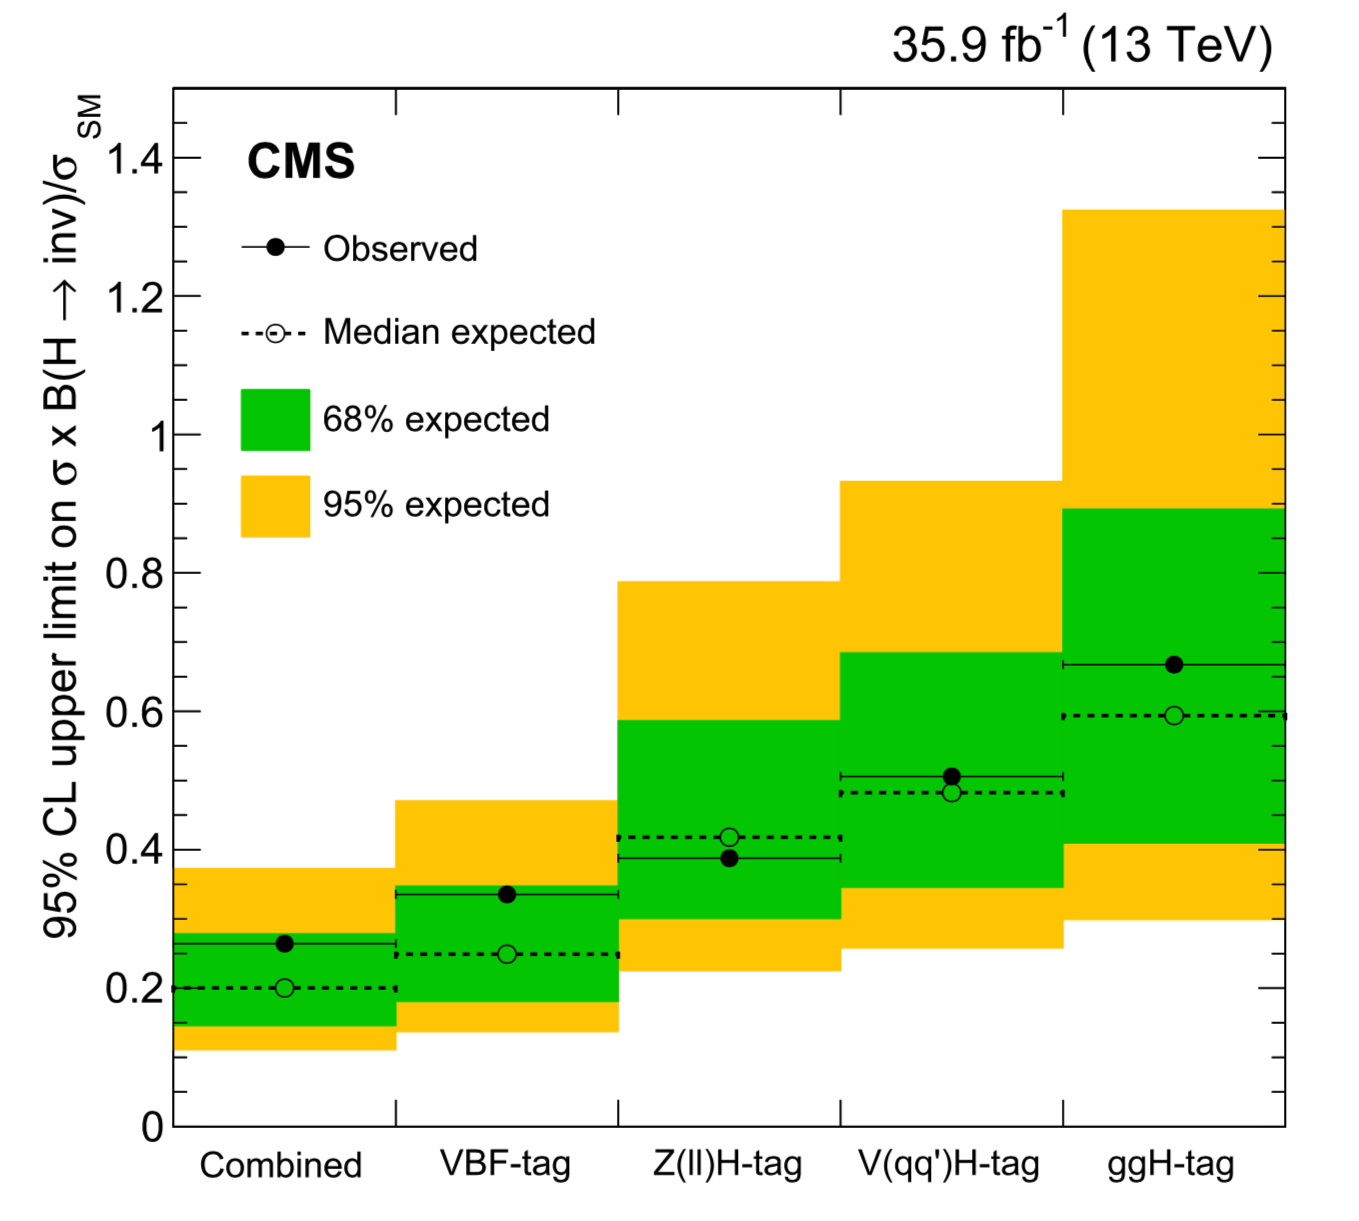
\includegraphics[width=0.7\textwidth]{Theory/Limit_2016.png}
        \caption{Summary of results from the CMS experiment for the 95\% CL upper limit on the $\sigma \times$~Br(H$\rightarrow$~inv)$/\sigma_{SM}$ under the assumption of the SM Higgs boson, for the 2016 era of data taking.~\cite{paper:HIG_17_023}.}
      \label{fig:limit_2016}
    \end{center}
  \end{figure}
 
\hspace{10pt} Continuing the story which began in Section~\ref{sec:dm}, these results can be interpreted in terms of the upper limit on the spin-independent DM-nucleon interaction cross section, making it easier to compare with direct detection experiments. The conversion can be made using the following relations (with the assumption of a scalar or a fermion DM particle respectively)~\cite{paper:hinv_run1,paper:hig_portal_models1}:

\begin{equation}
    \text{Br}(\text{H}\rightarrow \text{inv}) = \frac{\Gamma_{inv}}{\Gamma_{SM}+\Gamma_{inv}}
\end{equation}
\begin{equation}
    \sigma^{SI}_{Scalar-N} = \frac{4\Gamma_{inv}}{\beta m^3_Hv^2}\frac{f_N^2m_N^4}{(m_N+m_{DM})^2},
\label{eq:xs_scalar}    
\end{equation}
\begin{equation}
    \sigma^{SI}_{Fermion-N} = \frac{8\Gamma_{inv}m_{DM}^2}{\beta^3m^5_Hv^2}\frac{f_N^2m_N^4}{(m_N+m_{DM})^2},
\label{eq:xs_ferm}  
\end{equation}

where the values of the parameters are: $\Gamma_{SM} = $~4.07~MeV, $m_N = 0.939$~GeV (average mass of the proton and neutron), $v =$~246~GeV, the DM candidate's mass ($m_{DM}$), $\beta = \sqrt{1-\frac{4m_{DM}^2}{m_H^2}}$, and the $f_N=0.308$ (nuclear form-factor~\cite{paper:form_fact, paper:HIG_17_023}). One last important step is that the the main result, the Br(H$\rightarrow$inv) is expressed in terms of the 90~\% CL upper limit instead of the usual 95~\% in order to be comparable with the results presented by the direct detection experiments. Figure~\ref{fig:dm_2016} shows the comparison of the CMS experiment's results compared to results coming from direct detection experiments. These show that the approach taken by this analysis, covering $m_{DM}<\frac{m_H}{2}$, leads to a set of results complementing the majority of direct detection experiments. %avoiding the competition aspect while enhancing the affinity towards cooperation in order to achieve a better look at the overall picture.

\hspace{10pt} This chapter concludes the first part of this thesis which served as an introduction to main mechanisms of the SM and the motivation driving the search for the invisible final state of the Higgs boson. The following chapters introduce the experimental setup - the CMS experiment. There it will be presented how these measurements are made possible on the detector and trigger level. The continuation of this idea from the perspective of the newly available data is the focus of Chapter~\ref{ch:an_strategy} and beyond, where a combination of new trigger ideas and improved analysis strategy is discussed in great detail.

  \begin{figure}[htbp]
    \begin{center}
        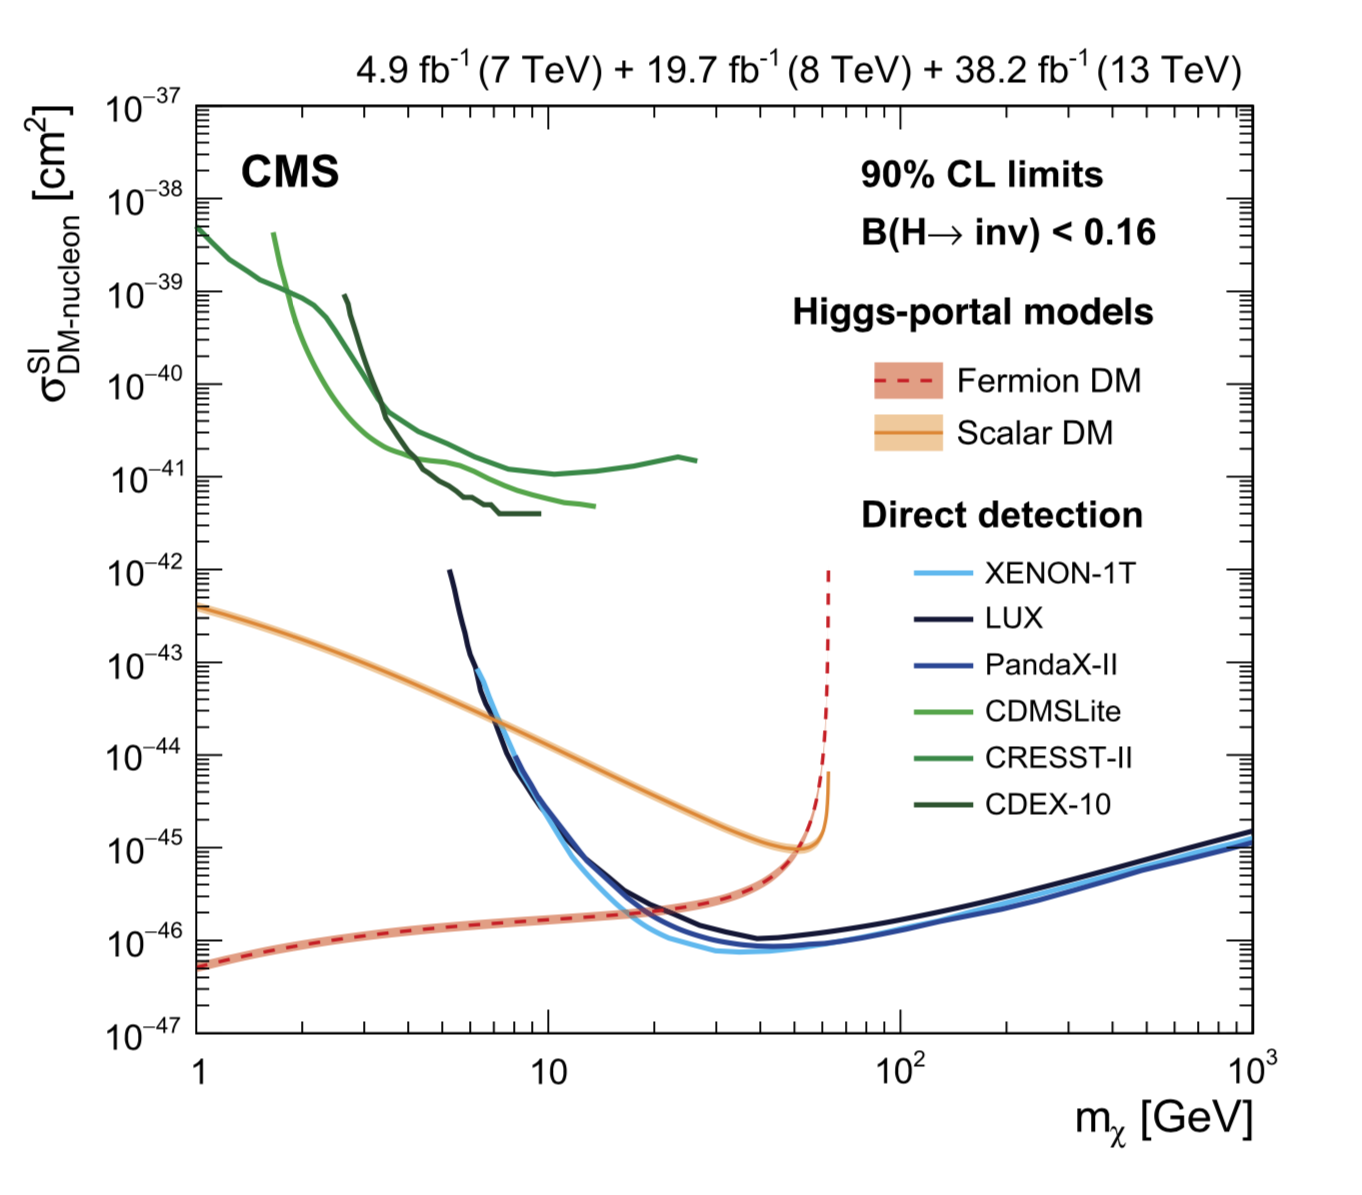
\includegraphics[width=0.75\textwidth]{Theory/DM_2016.png}
        \caption{The reinterpretation of the CMS results in terms of the 90\% CL upper limits on the spin-independent DM-nulcleon scattering cross section when assuming a fermion (red) or a scalar (orange) DM particle (presented as a function of $m_{DM}$, denoted here as $m_{\chi}$). Limits are compared with results originating from direct DM detection experiments~\cite{paper:HIG_17_023}.}
      \label{fig:dm_2016}
    \end{center}
  \end{figure}


 \tikzset{
    pgfornamentstyle/.style={scale=0.4}
  }
\begin{center}
    \expandafter\pgfornament\expandafter{88}
\end{center}
 \tikzset{
    pgfornamentstyle/.style={scale=1}
  }
\restoregeometry